\documentclass{beamer}
\usepackage{amsmath,graphics}
\usepackage{amssymb}

\usetheme{default}
\usepackage{xcolor}

\definecolor{solarizedBase03}{HTML}{002B36}
\definecolor{solarizedBase02}{HTML}{073642}
\definecolor{solarizedBase01}{HTML}{586e75}
\definecolor{solarizedBase00}{HTML}{657b83}
\definecolor{solarizedBase0}{HTML}{839496}
\definecolor{solarizedBase1}{HTML}{93a1a1}
\definecolor{solarizedBase2}{HTML}{EEE8D5}
\definecolor{solarizedBase3}{HTML}{FDF6E3}
\definecolor{solarizedYellow}{HTML}{B58900}
\definecolor{solarizedOrange}{HTML}{CB4B16}
\definecolor{solarizedRed}{HTML}{DC322F}
\definecolor{solarizedMagenta}{HTML}{D33682}
\definecolor{solarizedViolet}{HTML}{6C71C4}
%\definecolor{solarizedBlue}{HTML}{268BD2}
\definecolor{solarizedBlue}{HTML}{134676}
\definecolor{solarizedCyan}{HTML}{2AA198}
\definecolor{solarizedGreen}{HTML}{859900}
\definecolor{myBlue}{HTML}{162DB0}%{261CA4}
\setbeamercolor*{item}{fg=myBlue}
\setbeamercolor{normal text}{fg=solarizedBase03, bg=solarizedBase3}
\setbeamercolor{alerted text}{fg=myBlue}
\setbeamercolor{example text}{fg=myBlue, bg=solarizedBase3}
\setbeamercolor*{frametitle}{fg=solarizedRed}
\setbeamercolor*{title}{fg=solarizedRed}
\setbeamercolor{block title}{fg=myBlue, bg=solarizedBase3}
\setbeameroption{hide notes}
\setbeamertemplate{note page}[plain]
\beamertemplatenavigationsymbolsempty
\usefonttheme{professionalfonts}
\usefonttheme{serif}

\usepackage{fourier}

\def\vec#1{\mathchoice{\mbox{\boldmath$\displaystyle#1$}}
{\mbox{\boldmath$\textstyle#1$}}
{\mbox{\boldmath$\scriptstyle#1$}}
{\mbox{\boldmath$\scriptscriptstyle#1$}}}
\definecolor{OwnGrey}{rgb}{0.560,0.000,0.000} % #999999
\definecolor{OwnBlue}{rgb}{0.121,0.398,0.711} % #1f64b0
\definecolor{red4}{rgb}{0.5,0,0}
\definecolor{blue4}{rgb}{0,0,0.5}
\definecolor{Blue}{rgb}{0,0,0.66}
\definecolor{LightBlue}{rgb}{0.9,0.9,1}
\definecolor{Green}{rgb}{0,0.5,0}
\definecolor{LightGreen}{rgb}{0.9,1,0.9}
\definecolor{Red}{rgb}{0.9,0,0}
\definecolor{LightRed}{rgb}{1,0.9,0.9}
\definecolor{White}{gray}{1}
\definecolor{Black}{gray}{0}
\definecolor{LightGray}{gray}{0.8}
\definecolor{Orange}{rgb}{0.1,0.2,1}
\setbeamerfont{sidebar right}{size=\scriptsize}
\setbeamercolor{sidebar right}{fg=Black}

\renewcommand{\emph}[1]{{\textcolor{solarizedRed}{\itshape #1}}}

\newcommand\cA{\mathcal A}
\newcommand\cB{\mathcal B}
\newcommand\cC{\mathcal C}
\newcommand\cD{\mathcal D}
\newcommand\cE{\mathcal E}
\newcommand\cF{\mathcal F}
\newcommand\cG{\mathcal G}
\newcommand\cH{\mathcal H}
\newcommand\cI{\mathcal I}
\newcommand\cJ{\mathcal J}
\newcommand\cK{\mathcal K}
\newcommand\cL{\mathcal L}
\newcommand\cM{\mathcal M}
\newcommand\cN{\mathcal N}
\newcommand\cO{\mathcal O}
\newcommand\cP{\mathcal P}
\newcommand\cQ{\mathcal Q}
\newcommand\cR{\mathcal R}
\newcommand\cS{\mathcal S}
\newcommand\cT{\mathcal T}
\newcommand\cU{\mathcal U}
\newcommand\cV{\mathcal V}
\newcommand\cW{\mathcal W}
\newcommand\cX{\mathcal X}
\newcommand\cY{\mathcal Y}
\newcommand\cZ{\mathcal Z}

\newcommand\fA{\mathfrak A}
\newcommand\fB{\mathfrak B}
\newcommand\fC{\mathfrak C}
\newcommand\fD{\mathfrak D}
\newcommand\fE{\mathfrak E}
\newcommand\fF{\mathfrak F}
\newcommand\fG{\mathfrak G}
\newcommand\fH{\mathfrak H}
\newcommand\fI{\mathfrak I}
\newcommand\fJ{\mathfrak J}
\newcommand\fK{\mathfrak K}
\newcommand\fL{\mathfrak L}
\newcommand\fM{\mathfrak M}
\newcommand\fN{\mathfrak N}
\newcommand\fO{\mathfrak O}
\newcommand\fP{\mathfrak P}
\newcommand\fQ{\mathfrak Q}
\newcommand\fR{\mathfrak R}
\newcommand\fS{\mathfrak S}
\newcommand\fT{\mathfrak T}
\newcommand\fU{\mathfrak U}
\newcommand\fV{\mathfrak V}
\newcommand\fW{\mathfrak W}
\newcommand\fX{\mathfrak X}
\newcommand\fY{\mathfrak Y}
\newcommand\fZ{\mathfrak Z}

\newcommand\fa{\mathfrak a}
\newcommand\fb{\mathfrak b}
\newcommand\fc{\mathfrak c}
\newcommand\fd{\mathfrak d}
\newcommand\fe{\mathfrak e}
\newcommand\ff{\mathfrak f}
\newcommand\fg{\mathfrak g}
\newcommand\fh{\mathfrak h}
%\newcommand\fi{\mathfrak i}
\newcommand\fj{\mathfrak j}
\newcommand\fk{\mathfrak k}
\newcommand\fl{\mathfrak l}
\newcommand\fm{\mathfrak m}
\newcommand\fn{\mathfrak n}
\newcommand\fo{\mathfrak o}
\newcommand\fp{\mathfrak p}
\newcommand\fq{\mathfrak q}
\newcommand\fr{\mathfrak r}
\newcommand\fs{\mathfrak s}
\newcommand\ft{\mathfrak t}
\newcommand\fu{\mathfrak u}
\newcommand\fv{\mathfrak v}
\newcommand\fw{\mathfrak w}
\newcommand\fx{\mathfrak x}
\newcommand\fy{\mathfrak y}
\newcommand\fz{\mathfrak z}

\newcommand\vA{\vec A}
\newcommand\vB{\vec B}
\newcommand\vC{\vec C}
\newcommand\vD{\vec D}
\newcommand\vE{\vec E}
\newcommand\vF{\vec F}
\newcommand\vG{\vec G}
\newcommand\vH{\vec H}
\newcommand\vI{\vec I}
\newcommand\vJ{\vec J}
\newcommand\vK{\vec K}
\newcommand\vL{\vec L}
\newcommand\vM{\vec M}
\newcommand\vN{\vec N}
\newcommand\vO{\vec O}
\newcommand\vP{\vec P}
\newcommand\vQ{\vec Q}
\newcommand\vR{\vec R}
\newcommand\vS{\vec S}
\newcommand\vT{\vec T}
\newcommand\vU{\vec U}
\newcommand\vV{\vec V}
\newcommand\vW{\vec W}
\newcommand\vX{\vec X}
\newcommand\vY{\vec Y}
\newcommand\vZ{\vec Z}

\newcommand\va{\vec a}
\newcommand\vb{\vec b}
\newcommand\vc{\vec c}
\newcommand\vd{\vec d}
\newcommand\ve{\vec e}
\newcommand\vf{\vec f}
\newcommand\vg{\vec g}
\newcommand\vh{\vec h}
\newcommand\vi{\vec i}
\newcommand\vj{\vec j}
\newcommand\vk{\vec k}
\newcommand\vl{\vec l}
\newcommand\vm{\vec m}
\newcommand\vn{\vec n}
\newcommand\vo{\vec o}
\newcommand\vp{\vec p}
\newcommand\vq{\vec q}
\newcommand\vr{\vec r}
\newcommand\vs{\vec s}
\newcommand\vt{\vec t}
\newcommand\vu{\vec u}
\newcommand\vv{\vec v}
\newcommand\vw{\vec w}
\newcommand\vx{\vec x}
\newcommand\vy{\vec y}
\newcommand\vz{\vec z}

\renewcommand\AA{\mathbb A}
\newcommand\NN{\mathbb N}
\newcommand\ZZ{\mathbb Z}
\newcommand\PP{\mathbb P}
\newcommand\QQ{\mathbb Q}
\newcommand\RR{\mathbb R}
\renewcommand\SS{\mathbb S}
\newcommand\CC{\mathbb C}

\newcommand{\ord}{\mathrm{ord}}
\newcommand{\id}{\mathrm{id}}
\newcommand{\pr}{\mathrm{P}}
\newcommand{\Vol}{\mathrm{vol}}
\newcommand\norm[1]{\left\|{#1}\right\|} 
\newcommand\sign{\mathrm{sign}}
\newcommand{\eps}{\varepsilon}
\newcommand{\abs}[1]{\left|#1\right|}
\newcommand\bc[1]{\left({#1}\right)} 
\newcommand\cbc[1]{\left\{{#1}\right\}} 
\newcommand\bcfr[2]{\bc{\frac{#1}{#2}}} 
\newcommand{\bck}[1]{\left\langle{#1}\right\rangle} 
\newcommand\brk[1]{\left\lbrack{#1}\right\rbrack} 
\newcommand\scal[2]{\bck{{#1},{#2}}} 
\newcommand{\vecone}{\mathbb{1}}
\newcommand{\tensor}{\otimes}
\newcommand{\diag}{\mathrm{diag}}
\newcommand{\ggt}{\mathrm{ggT}}
\newcommand{\kgv}{\mathrm{kgV}}
\newcommand{\trans}{\top}

\newcommand{\Karonski}{Karo\'nski}
\newcommand{\Erdos}{Erd\H{o}s}
\newcommand{\Renyi}{R\'enyi}
\newcommand{\Lovasz}{Lov\'asz}
\newcommand{\Juhasz}{Juh\'asz}
\newcommand{\Bollobas}{Bollob\'as}
\newcommand{\Furedi}{F\"uredi}
\newcommand{\Komlos}{Koml\'os}
\newcommand{\Luczak}{\L uczak}
\newcommand{\Kucera}{Ku\v{c}era}
\newcommand{\Szemeredi}{Szemer\'edi}

\renewcommand{\ae}{\"a}
\renewcommand{\oe}{\"o}
\newcommand{\ue}{\"u}
\newcommand{\Ae}{\"A}
\newcommand{\Oe}{\"O}
\newcommand{\Ue}{\"U}

\newcommand{\mytitle}{Matrixrechnung}

\title[Linadi]{\mytitle}
\author[Amin Coja-Oghlan]{Amin Coja-Oghlan}
\institute[Frankfurt]{JWGUFFM}
\date{}

\begin{document}

\frame[plain]{\titlepage}

\begin{frame}\frametitle{\mytitle}
	\hfill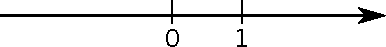
\includegraphics[height=10mm]{pics/reals.pdf}
	\begin{block}{Die reellen Zahlen}
		\begin{itemize}
			\item Mit $\RR$ wird die Menge der reellen Zahlen bezeichnet.
			\item Die reellen Zahlen k\oe nnen auf der Zahlengeraden abgetragen werden.
			\item Jede rationale Zahl ist eine reelle Zahl, also $\QQ\subset\RR$.
			\item Es gibt aber reelle Zahlen, die nicht rational sind.
			\item Beispiele: $\sqrt 2,\mathrm e,-\pi$.
		\end{itemize}
	\end{block}
\end{frame}

\begin{frame}\frametitle{\mytitle}
	\begin{block}{Die reellen Zahlen}
		\begin{itemize}
			\item Reelle Zahlen k\oe nnen durch als unendliche Dezimalentwicklung geschrieben werden, z.B.
				\begin{align*}
				\pi=3,141592\dots
				\end{align*}
			\item Die Dezimalentwicklung ist endlich oder periodisch genau dann, wenn es sich um eine rationale Zahl handelt, z.B.\
				\begin{align*}
					\frac54&=1.25&-\frac19&=-0.11111\dots
				\end{align*}
			\item Irrationale Zahlen k\oe nnen also nicht ohne weiteres im Computer dargestellt werden.
		\end{itemize}
	\end{block}
\end{frame}

\begin{frame}\frametitle{\mytitle}
	\begin{block}{Rechenregeln f\ue r reelle Zahlen}
		\begin{itemize}
			\item		Auf den reellen Zahlen stehen die Grundrechenarten $+,-,\,\cdot\,,\,/\,$ zur Verf\ue gung.
			\item  Es ist nicht ganz einfach, diese Rechenoperationen f\ue r unendliche Dezimalzahlen zu \emph{definieren}.
			\item Aber sie erf\ue llen dieselben Rechenregeln wie die Grundrechenarten f\ue r die rationalen Zahlen.
		\end{itemize}
	\end{block}
\end{frame}

\begin{frame}\frametitle{\mytitle}
	\begin{block}{Rechenregeln f\ue r reelle Zahlen}
		F\ue r die \emph{Addition} gelten folgende Regeln.
		\begin{description}
			\item[Kommutativgesetz:] $x+y=y+x$
			\item[Assoziativgesetz:] $(x+y)+z=x+(y+z)$
			\item[Neutrales Element:] $0+x=x$
			\item[Inverses Element:] zu jedem $x\in\RR$ existiert $y\in\RR$ mit $y+x=0$; wir schreiben $y=-x$.
		\end{description}
		Also bildet $(\RR,+)$ eine \emph{abelsche Gruppe}.
	\end{block}
\end{frame}

\begin{frame}\frametitle{\mytitle}
	\begin{block}{Rechenregeln f\ue r reelle Zahlen}
		F\ue r die \emph{Multiplikation} gelten folgende Regeln.
		\begin{description}
			\item[Kommutativgesetz:] $x\cdot y=y\cdot x$
			\item[Assoziativgesetz:] $(x\cdot y)\cdot z=x\cdot (y\cdot z)$
			\item[Neutrales Element:] $1\cdot x=x$
			\item[Inverses Element:] zu jedem $x\in\RR\setminus\cbc 0$ existiert $y\in\RR$ mit $y\cdot x=1$; wir schreiben $y=x^{-1}$.
		\end{description}
		Also bildet $(\RR\setminus\cbc 0,\,\cdot\,)$ eine \emph{abelsche Gruppe}.
	\end{block}
\end{frame}

\begin{frame}\frametitle{\mytitle}
	\begin{block}{Rechenregeln f\ue r reelle Zahlen}
		Die Multiplikation und die Addition verbindet das
		\begin{description}
			\item[Distributivgesetz:] $x\cdot(y+z)=x\cdot y+x\cdot z$
		\end{description}
	Mit anderen Worten bildet $(\RR,+,\,\cdot\,)$ einen \emph{K\oe rper}.
	\end{block}
\end{frame}

\begin{frame}\frametitle{\mytitle}
	\begin{block}{Rechenregeln f\ue r reelle Zahlen}
	\begin{itemize}
	\item Zus\ae tzlich besitzt $\RR$ die Vergleichsoperationen
		\begin{align*}
		<\qquad >\qquad \leq\qquad \geq
		\end{align*}
	\item Diese erf\ue llen die Eigenschaften
		\begin{align*}
			x&\geq y&\Rightarrow&&&x+z\geq y+z\\
			x&\geq 0\mbox{ und }y\geq 0&\Rightarrow&&&x\cdot y\geq0
		\end{align*}
	\end{itemize}
	\end{block}
\end{frame}

\begin{frame}\frametitle{\mytitle}
	\begin{block}{Definition}
		\begin{itemize}
			\item Eine \emph{$m\times n$-Matrix} ist ein rechteckiges Zahlschema
				\begin{align*}
					(a_{ij})_{\substack{1\leq i\leq m\\1\leq j\leq n}}=\begin{pmatrix}a_{11}&\cdots&a_{1n}\\\vdots&\ddots&\vdots\\a_{m1}&\cdots&a_{mn}\end{pmatrix}
				\end{align*}
				aus $m$ Zeilen und $n$ Spalten mit Eintr\ae gen $a_{ij}\in\RR$.
			\item \emph{Merke:} ``Zeilen zuerst, Spalten sp\ae ter''.
			\item Mit $\RR^{m\times n}$ wird die Menge aller $m\times n$-Matrizen bezeichnet.
		\end{itemize}
	\end{block}
\end{frame}

\begin{frame}\frametitle{\mytitle}
	\begin{block}{Beispiel}
		\begin{itemize}
			\item $1\times 1$-Matrizen sind einfach reelle Zahlen.
			\item einige $2\times 2$-Matrizen: 
				\begin{align*}
					\begin{pmatrix} -1&1\\2&0 \end{pmatrix}&&
					\begin{pmatrix} -\pi/2&\frac{3}{4}\\-\mathrm e^2&-19 \end{pmatrix}&&
					\begin{pmatrix} 1&0\\0&1\end{pmatrix}&&
					\begin{pmatrix} 0&0\\0&0\end{pmatrix}
				\end{align*}
			\item einige $2\times 1$-Matrizen und $1\times 2$-Matrizen:
				\begin{align*}
					\begin{pmatrix}1\\-1\end{pmatrix}&&
					\begin{pmatrix}\sqrt 2\\\frac{7}{9}\end{pmatrix}&&
					\begin{pmatrix}1&-1\end{pmatrix}&&
					\begin{pmatrix}\sqrt 2&\frac{7}{9}\end{pmatrix}
				\end{align*}
			\item einige gr\oe\ss ere Matrizen:
				\begin{align*}
					\begin{pmatrix}1&-1&0\\0&1&-1\\-1&0&1\end{pmatrix}&&
					\begin{pmatrix}1/2&1/3&1/4&1/5\\\sqrt 2&2&2^{3/2}&\sqrt 2\\0&0&0&0\end{pmatrix}
				\end{align*}
		\end{itemize}
	\end{block}
\end{frame}

\begin{frame}\frametitle{\mytitle}
	\begin{block}{Addition von Matrizen}
		\begin{itemize}
			\item Angenommen \begin{align*}
					A&=(a_{ij})_{\substack{1\leq i\leq m\\1\leq j\leq n}}&
					\mbox{und}&&
					B&=(b_{ij})_{\substack{1\leq i\leq m\\1\leq j\leq n}}
			\end{align*}
				sind zwei Matrizen derselben Gr\oe\ss e.
			\item Dann definieren wir die $m\times n$-Matrix
				\begin{align*}
					A+B&=(a_{ij}+b_{ij})_{\substack{1\leq i\leq m\\1\leq j\leq n}}.
				\end{align*}
			\item \emph{Matrizen werden eintragsweise addiert!}
		\end{itemize}
	\end{block}
\end{frame}

\begin{frame}\frametitle{\mytitle}
	\begin{block}{Beispiele}
		\begin{itemize}
			\item $\displaystyle\begin{pmatrix}1&2\\3&4\end{pmatrix}+\begin{pmatrix}5&6\\7&8\end{pmatrix}=\begin{pmatrix}6&8\\10&12\end{pmatrix}$
			\item $\displaystyle\begin{pmatrix}0&1\end{pmatrix}+\begin{pmatrix}0&-1\end{pmatrix}=\begin{pmatrix}0&0\end{pmatrix}$
			\item $\displaystyle\begin{pmatrix}0&1&2\\3&4&5\end{pmatrix}+\begin{pmatrix}0&0&0\\0&0&0\end{pmatrix}=\begin{pmatrix}0&1&2\\3&4&5\end{pmatrix}$
			\item $\displaystyle\begin{pmatrix}-1\\1\end{pmatrix}+\begin{pmatrix}-1\\1\end{pmatrix}=\begin{pmatrix}-2\\2\end{pmatrix}$
			\item Die Matrizen $\begin{pmatrix}1&2\\3&4\end{pmatrix}$ und $\begin{pmatrix}0&1&2\\3&4&5\end{pmatrix}$ k\oe nnen nicht addiert werden, weil sie verschiedene Gr\oe\ss en haben.
		\end{itemize}
	\end{block}
\end{frame}

\begin{frame}\frametitle{\mytitle}
	\begin{block}{Rechenregeln f\ue r die Addition von Matrizen}
		Angenommen $A=(a_{ij})_{i,j},B,C$ sind $m\times n$-Matrizen.
		\begin{description}
			\item[Kommutativgesetz:] $A+B=B+A$
			\item[Assoziativgesetz:] $(A+B)+C=A+(B+C)$
		\end{description}
	\end{block}
\end{frame}

\begin{frame}\frametitle{\mytitle}
	\begin{block}{Rechenregeln f\ue r die Addition von Matrizen}
		\begin{description}
			\item[Neutrales Element:] f\ue r die Nullmatrix
						\begin{align*}
							0&=\begin{pmatrix}
								0&\cdots&0\\\vdots&\ddots&\vdots\\0&\cdots&0
							\end{pmatrix}
						\end{align*}
				gilt $0+A=A$.
			\item[Inverses Element:] f\ue r die Matrix \begin{align*}
					-A=(-a_{ij})_{i,j}=\begin{pmatrix}-a_{11}&\cdots&-a_{1n}\\\vdots&\ddots&\vdots\\-a_{m1}&\cdots&-a_{mn}\end{pmatrix}
			\end{align*} gilt $(-A)+A=0$.
		\end{description}
	\emph{Die $m\times n$-Matrizen bilden mit der Addition eine Abelsche Gruppe.}
	\end{block}
\end{frame}

\begin{frame}\frametitle{\mytitle}
	\begin{block}{Beispiel}
		\begin{align*}
			-\begin{pmatrix} 1&2&3\\4&5&6 \end{pmatrix}&=\begin{pmatrix} -1&-2&-3\\-4&-5&-6 \end{pmatrix}
		\end{align*}
	\end{block}
\end{frame}

\begin{frame}\frametitle{\mytitle}
	\begin{block}{Multiplizieren von Matrizen}
		\begin{itemize}
		\item Sei $A=(a_{ij})_{i,j}$ eine $\ell\times m$-Matrix.
		\item Sei $B=(b_{ij})_{i,j}$ eine $m\times n$-Matrix.
		\item \emph{Beachte:} $B$ mu\ss\ soviele Zeilen haben, wie $A$ Spalten hat!
		\item Dann ist das Produkt $A\cdot B=C=(c_{hj})_{h,j}$ die $\ell\times n$-Matrix mit 
			\begin{align*}
				c_{hj}&=\sum_{i=1}^ma_{hi}b_{ij}&&(h=1,\ldots,\ell;\, j=1,\ldots,n)
			\end{align*}
		\item \emph{Merkregel:} ``Zeile mal Spalte''
		\end{itemize}
	\end{block}
\end{frame}

\begin{frame}\frametitle{\mytitle}
	\begin{block}{Multiplizieren von Matrizen}
		\begin{align*}
			C&=\begin{pmatrix}
				a_{11}b_{11}+\cdots+a_{1m}b_{m1}&\cdots&a_{11}b_{1n}+\cdots+a_{1m}b_{mn}\\
				\vdots&\ddots&\vdots\\
				a_{\ell1}b_{11}+\cdots+a_{\ell m}b_{m1}&\cdots&a_{\ell1}b_{1 n}+\cdots+a_{\ell m}b_{m n}
			\end{pmatrix}
			\end{align*}
			\begin{itemize}
				\item Es werden insgesamt $\ell\cdot m\cdot n$ Multiplikation von reellen Zahlen ausgef\ue hrt.
			\end{itemize}
		\end{block}
\end{frame}

\begin{frame}\frametitle{\mytitle}
	\begin{overprint}
	\onslide<1>
	\begin{block}{Beispiel}
		\begin{align*}
			\begin{pmatrix} 1&2\\3&4\end{pmatrix}\cdot	
			\begin{pmatrix} 5&6\\7&8\end{pmatrix}
							 &=
			\begin{pmatrix} 1\cdot 5+2\cdot 7&1\cdot 6+2\cdot 8\\3\cdot 5+4\cdot 7&3\cdot 6+4\cdot 8\end{pmatrix}
		= \begin{pmatrix} 19&22\\43&50\end{pmatrix}
		\end{align*}
	\end{block}
	\onslide<2>
	\begin{block}{Beispiel}
		\begin{align*}
			\begin{pmatrix} \textcolor{solarizedRed}{1}&\textcolor{solarizedRed}{2}\\3&4\end{pmatrix}\cdot	
			\begin{pmatrix} \textcolor{solarizedRed}{5}&6\\\textcolor{solarizedRed}{7}&8\end{pmatrix}
							 &=
			\begin{pmatrix} \textcolor{solarizedRed}{1\cdot 5+2\cdot 7}&1\cdot 6+2\cdot 8\\3\cdot 5+4\cdot 7&3\cdot 6+4\cdot 8\end{pmatrix}
			= \begin{pmatrix} \textcolor{solarizedRed}{19}&22\\43&50\end{pmatrix}
		\end{align*}
	\end{block}
	\onslide<3>
	\begin{block}{Beispiel}
		\begin{align*}
			\begin{pmatrix} \textcolor{solarizedRed}{1}&\textcolor{solarizedRed}{2}\\3&4\end{pmatrix}\cdot	
			\begin{pmatrix} 5&\textcolor{solarizedRed}{6}\\7&\textcolor{solarizedRed}{8}\end{pmatrix}
							 &=
			\begin{pmatrix} 1\cdot 5+2\cdot 7&\textcolor{solarizedRed}{1\cdot 6+2\cdot 8}\\3\cdot 5+4\cdot 7&3\cdot 6+4\cdot 8\end{pmatrix}
			= \begin{pmatrix} 19&\textcolor{solarizedRed}{22}\\43&50\end{pmatrix}
		\end{align*}
	\end{block}
	\onslide<4>
	\begin{block}{Beispiel}
		\begin{align*}
			\begin{pmatrix} 1&2\\\textcolor{solarizedRed}{3}&\textcolor{solarizedRed}{4}\end{pmatrix}\cdot	
			\begin{pmatrix} \textcolor{solarizedRed}{5}&6\\\textcolor{solarizedRed}{7}&8\end{pmatrix}
							 &=
			\begin{pmatrix} 1\cdot 5+2\cdot 7&1\cdot 6+2\cdot 8\\\textcolor{solarizedRed}{3\cdot 5+4\cdot 7}&3\cdot 6+4\cdot 8\end{pmatrix}
			= \begin{pmatrix} 19&22\\\textcolor{solarizedRed}{43}&50\end{pmatrix}
		\end{align*}
	\end{block}
	\onslide<5>
	\begin{block}{Beispiel}
		\begin{align*}
			\begin{pmatrix} 1&2\\\textcolor{solarizedRed}{3}&\textcolor{solarizedRed}{4}\end{pmatrix}\cdot	
			\begin{pmatrix} 5&\textcolor{solarizedRed}{6}\\7&\textcolor{solarizedRed}{8}\end{pmatrix}
							 &=
			\begin{pmatrix} 1\cdot 5+2\cdot 7&1\cdot 6+2\cdot 8\\3\cdot 5+4\cdot 7&\textcolor{solarizedRed}{3\cdot 6+4\cdot 8}\end{pmatrix}
			= \begin{pmatrix} 19&22\\43&\textcolor{solarizedRed}{50}\end{pmatrix}
		\end{align*}
	\end{block}
\end{overprint}
\end{frame}

\begin{frame}\frametitle{\mytitle}
	\begin{block}{Beispiel}
		\begin{align*}
			\begin{pmatrix} 0&1\\1&0\end{pmatrix}\cdot	
			\begin{pmatrix} 0&1\\0&0\end{pmatrix}
							 &=
			\begin{pmatrix} 0\cdot 0+1\cdot 0&0\cdot 1+1\cdot 0\\1\cdot 0+0\cdot 0&1\cdot 1+0\cdot 0\end{pmatrix}
		= \begin{pmatrix} 0&0\\0&1\end{pmatrix}\\
			\begin{pmatrix} 0&1\\0&0\end{pmatrix} \cdot	\begin{pmatrix} 0&1\\1&0\end{pmatrix}
							 &=
			\begin{pmatrix} 0\cdot 0+1\cdot 1&0\cdot 1+1\cdot 0\\0\cdot 0+0\cdot 1&0\cdot 1+0\cdot 0\end{pmatrix}
		= \begin{pmatrix} 1&0\\0&0\end{pmatrix}
		\end{align*}
	\emph{Die Matrixmultiplikation ist nicht kommutativ!}
	\end{block}
\end{frame}

\begin{frame}\frametitle{\mytitle}
	\begin{block}{Beispiel}
		\begin{align*}
			\begin{pmatrix} 0&1\\0&0\end{pmatrix}\cdot	
			\begin{pmatrix} 1&0\\0&0\end{pmatrix}
							 &=
			\begin{pmatrix} 0\cdot 1+1\cdot 0&0\cdot 0+1\cdot 0\\0\cdot 1+0\cdot 0&0\cdot 0+0\cdot 0\end{pmatrix}
		= \begin{pmatrix} 0&0\\0&0\end{pmatrix}
		\end{align*}
	\emph{Das Ergebnis der Multiplikation kann die Nullmatrix sein, obwohl beide Faktoren von Null verschieden sind!}
	\end{block}
\end{frame}

\begin{frame}\frametitle{\mytitle}
	\begin{block}{Beispiel}
		\begin{align*}
			\begin{pmatrix} 1&0\\0&1\end{pmatrix}\cdot	
			\begin{pmatrix} 1&2&3\\4&5&6\end{pmatrix}
							 &=
			\begin{pmatrix} 1\cdot 1+0\cdot 4&1\cdot 2+0\cdot 5&1\cdot 3+0\cdot 6\\0\cdot 1+1\cdot 4&0\cdot 2+1\cdot 5&0\cdot 3+1\cdot 6\end{pmatrix}\\
											 &= \begin{pmatrix} 1&2&3\\4&5&6\end{pmatrix}
		\end{align*}
	\end{block}
\end{frame}

\begin{frame}\frametitle{\mytitle}
	\begin{block}{Beispiel}
		\begin{align*}
			\begin{pmatrix} 2&0\\0&2\end{pmatrix}\cdot	
			\begin{pmatrix} 1&2&3\\4&5&6\end{pmatrix}
							 &=
			\begin{pmatrix} 2\cdot 1+0\cdot 4&2\cdot 2+0\cdot 5&2\cdot 3+0\cdot 6\\0\cdot 1+2\cdot 4&0\cdot 2+2\cdot 5&0\cdot 3+2\cdot 6\end{pmatrix}\\
											 &= \begin{pmatrix} 2&4&6\\8&10&12\end{pmatrix}
		\end{align*}
	\end{block}
\end{frame}

\begin{frame}\frametitle{\mytitle}
	\begin{block}{Beispiel}
		\begin{align*}
			\begin{pmatrix} 1&-1\\1&0\end{pmatrix}\cdot	
			\begin{pmatrix} 2\\4\end{pmatrix}
							 &=
			\begin{pmatrix}1\cdot 2-1\cdot4\\1\cdot 2+0\cdot 4\end{pmatrix}=
				\begin{pmatrix} -2\\2\end{pmatrix}\\
			\begin{pmatrix} 2&4\end{pmatrix}\cdot	
			\begin{pmatrix} 1&-1\\1&0\end{pmatrix}
							 &=
							 \begin{pmatrix}2\cdot 1+4\cdot1&2\cdot (-1)+4\cdot 0\end{pmatrix}=
							 \begin{pmatrix}6&-2\end{pmatrix}
		\end{align*}
	\end{block}
\end{frame}

\begin{frame}\frametitle{\mytitle}
	\begin{block}{Beispiel}
		\begin{align*}
			\begin{pmatrix} 1&-1 \end{pmatrix}\cdot \begin{pmatrix} 3\\3 \end{pmatrix}&=1\cdot 3-1\cdot 3=0\\
			\begin{pmatrix} 1\\-1 \end{pmatrix}\cdot \begin{pmatrix} 3&3 \end{pmatrix}&=
			\begin{pmatrix} 1\cdot 3&1\cdot 3\\-1\cdot 3&-1\cdot 3 \end{pmatrix} 
			=		\begin{pmatrix} 3&3\\-3&-3 \end{pmatrix} 
		\end{align*}
	\end{block}
\end{frame}

\begin{frame}\frametitle{\mytitle}
	\begin{block}{Diagonalmatrizen}
		\begin{itemize}
			\item Eine $n\times n$-Matrix $A=(a_{ij})_{i,j=1,\ldots,n}$ hei\ss t eine \emph{Diagonalmatrix}, falls $a_{ij}=0$ f\ue r alle $i,j\in\{1,\ldots,n\}$ mit $i\neq j$.
		\item Mit anderen Worten: nur die $n$ Diagonaleintr\ae ge $$a_{11},a_{22},\ldots,a_{nn}$$ d\ue rfen von Null verschieden sein.
		\item F\ue r gegebene Zahlen $d_1,\ldots,d_n$ bezeichnet
			$$\diag(d_1,\ldots,d_n)$$
			die Diagonalmatrix mit den Diagonaleintr\ae gen $d_1,\ldots,d_n$.
		\end{itemize}
	\end{block}
\end{frame}

\begin{frame}\frametitle{\mytitle}
	\begin{block}{Die Identit\ae tsmatrix}
		\begin{itemize}
			\item Die $n\times n$-Diagonalmatrix
				\begin{align*}
					\diag(\underbrace{1,\ldots,1}_{\mbox{ n mal}})
				\end{align*}
				hei\ss t die \emph{$n\times n$-Identit\ae tsmatrix}.
			\item Sie wird durch $\id_n$ bezeichnet.
			\item Wenn $n$ bekannt ist, schreiben wir einfach $\id$.
		\end{itemize}
	\end{block}
\end{frame}

\begin{frame}\frametitle{\mytitle}
	\begin{block}{Rechenregeln f\ue r die Matrixmultiplikation}
Seien $A,B,C$ Matrizen der Gr\oe\ss en $\ell\times m$, $m\times n$ und $n\times p$.
		\begin{description}
			\item[Assoziativgesetz:] $(A\cdot B)\cdot C=A\cdot(B\cdot C)$.
			\item[Neutrales Element:] $\id_\ell\cdot A=A$ und $A\cdot\id_m=A$.
		\end{description}
		\emph{Die Matrixmultiplikation ist nicht kommutativ und nicht jede Matrix hat ein multiplikatives Inverses!}
	\end{block}
\end{frame}

\begin{frame}\frametitle{\mytitle}
	\begin{block}{Rechenregeln f\ue r die Matrizen}
Seien $A,B,C,D$ Matrizen der Gr\oe\ss en $\ell\times m$, $m\times n$, $m\times n$ und $n\times p$.
		\begin{description}
			\item[Distributivgesetz:] es gilt 
				\begin{align*}
					A\cdot(B+C)&=A\cdot B+A\cdot C\\
					(B+C)\cdot D&=B\cdot D+C\cdot D
				\end{align*}
		\end{description}
	\end{block}
\end{frame}

\begin{frame}\frametitle{\mytitle}
	\begin{block}{Proposition}
		F\ue r jede nat\ue rliche Zahl $n$ bildet die Menge $\RR^{n\times n}$ der $n\times n$-Matrizen mit den Operationen $+$ und $\,\cdot\,$ einen Ring.
	\end{block}
\end{frame}

\begin{frame}\frametitle{\mytitle}
	\begin{block}{Potenzieren von Matrizen}
	\begin{itemize}
	\item Sei $A$ eine $n\times n$-Matrix und $\ell\in\NN$.
	\item Weil $\RR^{n\times n}$ ein Ring ist, definieren wir
		\begin{align*}
			A^\ell&=\underbrace{A\cdot\ \cdots\ \cdot A}_{\mbox{$\ell$ mal}}
		\end{align*}
	\item Beispielsweise ist $A^2=A\cdot A$, $A^3=A\cdot A\cdot A$
	\item \emph{Konvention:} $A^0=\id_n$
	\end{itemize}
	\end{block}
\end{frame}

\begin{frame}\frametitle{\mytitle}
	\begin{block}{Multiplikation von Matrizen mit Skalaren}
		\begin{itemize}
			\item Angenommen $A=(a_{ij})_{i,j}$ ist eine $m\times n$-Matrix.
			\item Sei ferner $c\in\RR$.
			\item Wir definieren
				\begin{align*}
					c\cdot A&=\diag(\underbrace{c,\ldots,c}_{\mbox{ m mal}})\cdot A=\begin{pmatrix}
							   c\cdot a_{11}&\cdots&c\cdot a_{1n}\\\vdots&\ddots&\vdots\\c\cdot a_{m1}&\cdots&c\cdot a_{mn}
						   \end{pmatrix}
				\end{align*}
			\item Jeder Eintrag von $A$ wird also mit $c$ multipliziert.
			\item Die Rechenregeln f\ue r die Matrixmultiplikation \ue bertragen sich auf die Multiplikation mit Skalaren.
		\end{itemize}
	\end{block}
\end{frame}

\begin{frame}\frametitle{\mytitle}
	\begin{block}{Beispiel}
		\begin{align*}
			-3\cdot\begin{pmatrix}1&2\\3&4\end{pmatrix}&=\begin{pmatrix}-3&-6\\-9&-12\end{pmatrix}
		\end{align*}
	\end{block}
\end{frame}

\begin{frame}\frametitle{\mytitle}
	\begin{block}{Definition (transponierte Matrix)}
		\begin{itemize}
			\item Sei $A=(a_{ij})_{i,j}$ eine $m\times n$-Matrix.
			\item Die \emph{transponierte Matrix} $A^\trans$ ist die $n\times m$-Matrix
				\begin{align*}
					A^\trans&=(a_{ji})_{\substack{j=1,\ldots,n\\i=1,\ldots,m}}
					=\begin{pmatrix}
						a_{11}&\cdots&a_{m1}\\\vdots&\ddots&\vdots\\a_{1n}&\cdots&a_{mn}
					\end{pmatrix}
				\end{align*}
			\item \emph{$A^\trans$ ensteht aus $A$ durch Spiegeln an der Diagonalen.}
		\end{itemize}
	\end{block}
\end{frame}

\begin{frame}\frametitle{\mytitle}
	\begin{block}{Beispiele}
		\begin{align*}
			\begin{pmatrix} 1&2&3\\4&5&6 \end{pmatrix}^\trans&=
			\begin{pmatrix} 1&4\\2&5\\3&6 \end{pmatrix}\\
			\begin{pmatrix} 1\\2\\3 \end{pmatrix}^\trans&=\begin{pmatrix} 1&2&3\end{pmatrix}\\
			\begin{pmatrix} 1&0\\0&1 \end{pmatrix}^\trans&=\begin{pmatrix} 1&0\\0&1 \end{pmatrix}
		\end{align*}
	\end{block}
\end{frame}

\begin{frame}\frametitle{\mytitle}
	\begin{block}{Zusammenfassung}
		\begin{itemize}
			\item Matrizen sind rechteckige Zahlschemata
			\item Addition\item Multiplikation\item Multiplikation mit Skalaren
			\item Transposition
		\end{itemize}
	\end{block}
\end{frame}

\end{document}
